%%
%% UW CBE Thesis: thesis.tex
%% Written by Ankur Gupta, Sep 1, 2013
%% Departament of Chemical and Biological Engineering
%% University of Wisconsin-Madison
%% Copyright (c) Ankur Gupta, 2014
%%
%% License: GPL v3. See LICENSE.
%% UW CBE Thesis main .tex file
%%

\documentclass[11pt,oneside]{uwcbethesis}

%% Packages to be loaded
\usepackage{amsmath}	% Provides \align
\usepackage{graphicx}	% Provides \includegraphics
\usepackage{setspace}	% Provides \doublespacing
\usepackage[square,numbers]{natbib}	% Don't change this. See \citea{} in shortcuts.tex
\usepackage{subcaption}	% subfigures
% \usepackage{footnote} % Provides \footnote
% \usepackage[super,longnamesfirst]{natbib}
\usepackage{amssymb}	% Provides \because
\usepackage{amsthm}	% Enhanced theorem, definition, proof environments from the AMS


\usepackage[chapter]{algorithm}	% Provides algorithm environment. Algorithms will be referenced as [chapter]number.algorithmnumber
\usepackage{algpseudocode}	% Provides algorithmicx environment
\usepackage{booktabs} 	% Fancy tables. \toprule, \midrule, \bottomrule commands
\usepackage{threeparttable} % Provides threeparttable enviroment



% Define environments (requires amsthm)
% I need enviroments to be numbered as [chapter]number.[]number (just like equations).
\newtheorem{defn}{Definition}[chapter] 
\newtheorem{prop}{Proposition}[chapter]
\newtheorem{thm}{Theorem}
\newtheorem{lemma}[thm]{Lemma}
\newtheorem{assump}{Assumption}[chapter]


%% Load the commands/shortcuts
%%
%% UW CBE Thesis: uwcbethesis-config.tex
%% Written by Ankur Gupta, Sep 1, 2013
%% Departament of Chemical and Biological Engineering
%% University of Wisconsin-Madison
%% Copyright (c) Ankur Gupta, 2014
%%
%% License: GPL v3. See LICENSE.
%%

%% This file is where you store all commands.
%% Loads package which are absolutely required.
%% Does not load non-essential packages which you can load from thesis.tex
%%


%-----------------------------------------------------------------------------
%% User data:
% Name
\newcommand{\myName}{First Last\xspace}
% \newcommand{\myShortName}{F. Last\xspace}
% \newcommand{\myInitials}{F.L.\xspace}

% Title
\newcommand{\myTitle}{Full thesis title\xspace}
% \newcommand{\myShortTitle}{Short title\xspace}

% Degree and Subject
\newcommand{\myDegree}{Doctor of Philosophy\xspace}
% \newcommand{\myShortDegree}{Ph.D.\xspace}
\newcommand{\mySubject}{Chemical Engineering\xspace}

% Defense time
\newcommand{\myYear}{YYYY\xspace} % YYYY = year
\newcommand{\myMonth}{Month\xspace}
\newcommand{\myDate}{DD\xspace} % DD = day of the month
% \newcommand{\myDefenseDate}{10/15/2013\xspace}

% University
\newcommand{\myDepartment}{Full Department Name\xspace}
\newcommand{\myUniversity}{Full University Name\xspace}
\newcommand{\myLocation}{City, ST\xspace} % ST = State abbreviation

% Advisors and committee members
% Advisor
\newcommand{\myAdvisor}{Advisor Name\xspace}
\newcommand{\myAdvisorPos}{Professor\xspace}
\newcommand{\myAdvisorDep}{Short Department Name\xspace}
% Co-Advisor
\newcommand{\myCoAdvisor}{CoAdvisor Name\xspace}
\newcommand{\myCoAdvisorPos}{Professor\xspace}
\newcommand{\myCoAdvisorDep}{Short Department Name\xspace}
% Committee Member 1
\newcommand{\myCMemberOne}{Committee MemberOne\xspace}
\newcommand{\myCMemberOnePos}{Associate Professor\xspace}
\newcommand{\myCMemberOneDep}{Short Department Name\xspace}
% Committee Member 2
\newcommand{\myCMemberTwo}{Committee MemberTwo\xspace}
\newcommand{\myCMemberTwoPos}{Associate Professor\xspace}
\newcommand{\myCMemberTwoDep}{Short Department Name\xspace}
% Committee Member 3
\newcommand{\myCMemberThree}{Committee MemberThree\xspace}
\newcommand{\myCMemberThreePos}{Associate Professor\xspace}
\newcommand{\myCMemberThreeDep}{Short Department Name\xspace}
% Committee Member 4
\newcommand{\myCMemberFour}{Committee MemberFour\xspace}
\newcommand{\myCMemberFourPos}{Assistant Professor\xspace}
\newcommand{\myCMemberFourDep}{Short Department Name\xspace}
%-----------------------------------------------------------------------------


%-----------------------------------------------------------------------------
%% Packages which are used by this file
% Xspace: provides \xspace used above
\usepackage{xspace}
%-----------------------------------------------------------------------------


%-----------------------------------------------------------------------------
%% Frequently used commands
% Colors
% \newcommand{\maroon}[1]{\textcolor{Maroon}{#1}}

% Shortcuts
%%
%% UW CBE Thesis: shortcuts.tex
%% Written by Ankur Gupta, Sep 1, 2013
%% Departament of Chemical and Biological Engineering
%% University of Wisconsin-Madison
%% Copyright (c) Ankur Gupta, 2014
%%
%% License: GPL v3. See LICENSE.
%%


% Shortcuts.tex

% Chapter Shortcuts
% Name shortcuts using names that you can remember
% Example: Use \litsurvey instead of \chaptertwo
% You can use them throughout the thesis like this:
% \litsurvey{} presents a literature survey of the current research methodologies.
\newcommand{\intro}{Chapter~\ref{chap:intro}} % Introduction is Chapter 1
\newcommand{\chaptertwoname}{Chapter~\ref{chap:chaptertwoname}}
\newcommand{\chapterthreename}{Chapter~\ref{chap:chapterthreename}}
\newcommand{\chapterfourname}{Chapter~\ref{chap:chapterfourname}}
\newcommand{\chapterfivename}{Chapter~\ref{chap:chapterfivename}}
\newcommand{\conc}{Chapter~\ref{chap:conclusions}}
\newcommand{\appA}{Appendix~\ref{app:A}}

% Section reference
\newcommand{\mysec}[1]{Section~\ref{#1}}
\newcommand{\mysecs}[2]{Sections~\ref{#1} and~\ref{#2}}

% Equation shortcuts
\newcommand{\myeq}[1]{Eq.~\eqref{#1}}
\newcommand{\myeqr}[2]{Eqs.~\eqref{#1}-\eqref{#2}} % Range
\newcommand{\myeqs}[3]{Eqs.~\eqref{#1},~\eqref{#2},~\eqref{#3}}

% Figures shortcuts
\newcommand{\myfig}[1]{Figure~\ref{#1}}
\newcommand{\myfigr}[2]{Figures~\ref{#1}-\ref{#2}} % Range
\newcommand{\myfigs}[3]{Figures~\ref{#1},~\ref{#2},~\ref{#3}}

% Tables shortcuts
\newcommand{\mytab}[1]{Table~\ref{#1}}
\newcommand{\mytabr}[2]{Tables~\ref{#1}-\ref{#2}} % Range
\newcommand{\mytabs}[3]{Tables~\ref{#1},~\ref{#2},~\ref{#3}}

% Algorithm reference
\newcommand{\myalgo}[1]{Algorithm~\ref{#1}}


% Frequently used abbreviations
\newcommand{\ie}{\emph{i.\,e.}}
\newcommand{\Ie}{\emph{I.\,e.}}
\newcommand{\eg}{\emph{e.\,g.}}
\newcommand{\Eg}{\emph{E.\,g.}}

%%% MATH SHORTCUTS %%%
% Lowercase bolds
\newcommand{\bfx}{\mathbf{x}}
\newcommand{\bfy}{\mathbf{y}}
\newcommand{\bfr}{\mathbf{r}}
\newcommand{\bfz}{\mathbf{z}}
\newcommand{\bfv}{\mathbf{v}}
\newcommand{\bff}{\mathbf{f}}
\newcommand{\bfh}{\mathbf{h}}

% Uuppercase bolds
\newcommand{\bfX}{\mathbf{X}}
\newcommand{\bfY}{\mathbf{Y}}
\newcommand{\bfZ}{\mathbf{Z}}
\newcommand{\bfP}{\mathbf{P}}
\newcommand{\bfQ}{\mathbf{Q}}
\newcommand{\bfR}{\mathbf{R}}
\newcommand{\bfI}{\mathbf{I}}
\newcommand{\bfC}{\mathbf{C}}
\newcommand{\bfV}{\mathbf{V}}
\newcommand{\bfS}{\mathbf{S}}
\newcommand{\bfH}{\mathbf{H}}
\newcommand{\bfzero}{\mathbf{0}}

% Fancy mathcals (for reactions)
\newcommand{\fR}{\mathcal{R}}
\newcommand{\fX}{\mathcal{X}}
\newcommand{\fS}{\mathcal{S}}
\newcommand{\fN}{\mathcal{N}}

% Number systems and sets
\newcommand{\bbR}{\mathbb{R}}
\newcommand{\bbZ}{\mathbb{Z}}
\newcommand{\bbN}{\mathbb{N}}
\newcommand{\bbQ}{\mathbb{Q}}
\newcommand{\bbS}{\mathbb{S}}
\newcommand{\bbA}{\mathbb{A}}
\newcommand{\bbE}{\mathbb{E}}

\newcommand{\abs}[1]{\left| #1 \right|} % cardinality or absolute value



%-----------------------------------------------------------------------------



%-----------------------------------------------------------------------------
%% hyperref: So I can jump around in the PDF
\usepackage[pdftex,hyperfootnotes=false,pdfpagelabels]{hyperref}
\hypersetup{
    colorlinks=true, linktocpage=true, pdfstartpage=1, pdfstartview={FitH},
    breaklinks=true, pdfpagemode=UseNone, pageanchor=true, pdfpagemode=UseOutlines,
    plainpages=false, bookmarksnumbered, bookmarksopen=true, bookmarksopenlevel=1,
    hypertexnames=true, pdfhighlight=/O,%nesting=true,%frenchlinks,
    urlcolor=webbrown, linkcolor=RoyalBlue, citecolor=webgreen, %pagecolor=RoyalBlue,
    pdftitle={\myTitle},
    pdfauthor={\textcopyright\ \myName},
    pdfsubject={Chemical Engineering, Applied Mathematics, Systems Biology, Statistics},
    pdfkeywords={stochastic kinetic model, markov chains, importance sampling, ordinary differential equation},
    pdfcreator={pdfLaTeX},
    pdfproducer={LaTeX with hyperref and uwcbethesis}
}
\usepackage[all]{hypcap} % Makes sure that link to figure/table shows the figure/table instead of the caption
%-----------------------------------------------------------------------------


%-----------------------------------------------------------------------------
%% Index package: I want it
\usepackage{makeidx}
\makeindex
%-----------------------------------------------------------------------------


%-----------------------------------------------------------------------------
%% 'code' is shorter than verbatim
\usepackage{fancyvrb}
\DefineShortVerb{\|}
\VerbatimFootnotes
\DefineVerbatimEnvironment{code}{Verbatim}
{
    frame=single,
    framesep=0.25em,
    xleftmargin=1em,
    xrightmargin=1em,
    samepage=true,
    fontsize=\footnotesize
}
%-----------------------------------------------------------------------------

% \newcounter{dummy}



%% Adjustments to uwcbethesis-config (this should be after inputting uwcbethesis-config)
% Uncomment these two lines below for printing. Comment them for a screen version of the PDF.
% \hypersetup{colorlinks=false} % Puts boxes around the links. Links still work.
% \hypersetup{hidelinks} % Makes all links black. Links still work. 


\begin{document}
%---------------------------------------------
%% Front Matter
% Uncomment the following line when you're in draft mode. Comment out in the final version.
% %%
%% UW CBE Thesis: frontmatter/DraftTitlePage.tex
%% Written by Ankur Gupta, Sep 1, 2013
%% Departament of Chemical and Biological Engineering
%% University of Wisconsin-Madison
%% Copyright (c) Ankur Gupta, 2014
%%
%% License: GPL v3. See LICENSE.
%%

%% Inclusion of this page violated UW-Madison requirements.
%% This page is to mark the time/version of thesis draft.
%% Remove when finalized.
%%


% Don't need a page number
\thispagestyle{empty}


\begin{center}

\spacedlowsmallcaps{\myName}
\\
\medskip
\textcolor{Maroon}{\spacedallcaps{\myTitle}}

\end{center}


% This page should end now
\cleardoublepage % Does NOT require user editing.
%%
%% UW CBE Thesis: frontmatter/TitlePage.tex
%% Written by Ankur Gupta, Sep 1, 2013
%% Departament of Chemical and Biological Engineering
%% University of Wisconsin-Madison
%% Copyright (c) Ankur Gupta, 2014
%%
%% License: GPL v3. See LICENSE.
%%

%% UW requirement: Format similar to the sample title page
%% 		           PDF (most likely made in MSWord) that UW provides.
%%

% Add a PDF bookmark. Need to do this because this page is not in TOC
\pdfbookmark[1]{Title}{titlepagepdfmark}

% Reduce margins to fit all the text
\newgeometry{left=1.25in,right=1.25in,top=1in,bottom=1in}

% UW requirement: No page number (not even roman)
\thispagestyle{empty}

\vfill

\begin{center}
	\large
	\textcolor{Maroon}{\spacedallcaps{\myTitle}} \\
	\vspace{7ex}
	by \\
	\vspace{2ex}
	{\Large \spacedlowsmallcaps{\myName}} \\
	
	\vspace{9ex}
	
	A dissertation submitted in partial fulfillment of \\
	the requirements for the degree of \\
	
	\vspace{10ex}
	
	\myDegree \\
	\vspace{1ex}
	(\mySubject )\\
	
	\vspace{12ex}
	
	at the \\
	\vspace{1ex}
	\MakeTextUppercase{\myUniversity} \\
	\vspace{1ex}
	\myYear \\
\end{center}

\vspace{12ex}
\begin{flushleft}
Date of final oral examination: \myMonth \myDate , \myYear \\
\vspace{1ex}
The dissertation is approved by the following members of the Final Oral Committee:
\end{flushleft}

% Edit this only if you have different number of advisors, co-advisors or committee members.
% Don't hardcode names here. Use uwcbethesis-config.tex for these commands. 
\indent\indent \myAdvisor, \myAdvisorPos \myAdvisorDep \\
\indent\indent \myCoAdvisor, \myCoAdvisorPos, \myCoAdvisorDep \\
\indent\indent \myCMemberOne, \myCMemberOnePos, \myCMemberOneDep \\
\indent\indent \myCMemberTwo, \myCMemberTwoPos, \myCMemberTwoDep \\
\indent\indent \myCMemberThree, \myCMemberThreePos, \myCMemberThreeDep \\
\indent\indent \myCMemberFour, \myCMemberFourPos, \myCMemberFourDep \\
% \end{flushleft}

% This page should end now
\cleardoublepage

% Restore geometry defined in uwcbethesis.cls
\restoregeometry 
%%
%% UW CBE Thesis: frontmatter/CopyrightPage.tex
%% Written by Ankur Gupta, Sep 1, 2013
%% Departament of Chemical and Biological Engineering
%% University of Wisconsin-Madison
%% Copyright (c) Ankur Gupta, 2014
%%
%% License: GPL v3. See LICENSE.
%%

%% UW requirement: Copyright page is not necessary
%%                 but if inserted, it should be 
%% 		           directly after the title page.
%%
%% This file does not need user editing unless you want to change 
%% spacing, positioning etc. To change then names and other data
%% edit uwcbethesis-config.tex.

% Add a PDF bookmark. Need to do this because this page is not in TOC
\pdfbookmark[1]{Copyright}{copyright}

% UW requirement: No page number (not even roman)
\thispagestyle{empty}


% UW requirement: Center the text within the bottom third
%                 page within the margins

\hfill

\vfill

\begin{center}
\textcopyright\xspace Copyright by \myName \myYear\\
All Rights Reserved
\end{center}


% This page should end now
\cleardoublepage % Does NOT require user editing.
\pagenumbering{roman}
%%
%% UW CBE Thesis: frontmatter/DedicationPage.tex
%% Written by Ankur Gupta, Sep 1, 2013
%% Departament of Chemical and Biological Engineering
%% University of Wisconsin-Madison
%% Copyright (c) Ankur Gupta, 2014
%%
%% License: GPL v3. See LICENSE.
%%

%% Dedication page (dedication page if present should have number i)
%%

% Add a PDF bookmark. Need to do this because this page is not in TOC
\pdfbookmark[1]{Dedication}{dedication}

\vspace*{3cm}
\begin{center}
% Edit the line below
To the important person in my life who helped me. \\ \medskip
\end{center}


% This page should end now
\cleardoublepage % Requires user editing.
%%
%% UW CBE Thesis: frontmatter/AcksPage.tex
%% Written by Ankur Gupta, Sep 1, 2013
%% Departament of Chemical and Biological Engineering
%% University of Wisconsin-Madison
%% Copyright (c) Ankur Gupta, 2014
%%
%% License: GPL v3. See LICENSE.
%%

% Add a PDF bookmark. Need to do this because this page is not in TOC
\pdfbookmark[1]{Acknowledgments}{acknowledgements}

% \begin{flushright}{\slshape    
%     Essentially, all models are wrong, but some are useful.} \\ \medskip
%     --- \defcitealias{box:draper:1986}{George E. P. Box}\citetalias{box:draper:1986} \citep{box:draper:1986}
% \end{flushright}

\bigskip

% This is required to keep the quote above and the text below on the same page
\begingroup
\let\clearpage\relax
\let\cleardoublepage\relax
\let\cleardoublepage\relax

\chapter*{Acknowledgments}
% Write from your heart, young Jedi. 
I hereby acknowledge everybody who has helped me achieve my doctoral degree.\\


I thank my advisor. I thank my committee.\\

I thank my group members. \\

I thank my personal friends in the city. \\

I thank my family. \\

Finally, if I missed someone, I'm sorry. \\
\bigskip

\begin{flushright}
\myName \\
\myLocation \\
\myMonth \myYear
\end{flushright}

\endgroup 

% This page should end now
\cleardoublepage % Requires user editing.
%%
%% UW CBE Thesis: frontmatter/ContentsPage.tex
%% Written by Ankur Gupta, Sep 1, 2013
%% Departament of Chemical and Biological Engineering
%% University of Wisconsin-Madison
%% Copyright (c) Ankur Gupta, 2014
%%
%% License: GPL v3. See LICENSE.
%%

%% Please DO NOT edit these unless you know what you're doing. 
%% You've been warned. 


%------------------------------------------------------
%% Table of Contents
% Add to PDF bookmark list in the left hand side pane. 
% If you add to contents then you don't need to do a pdfbookmark
% \refstepcounter{dummy}
\pdfbookmark[1]{\contentsname}{tableofcontents} %the text tableofcontents could be any label in this command

% How many levels to number and display?
\setcounter{tocdepth}{2} % Do not list subsubsections and below
\setcounter{secnumdepth}{2} % Do not number subsubsections and below

% Format 'Contents' text
% \manualmark % Porbably belongs to scrpage2 package which I don't use
% \markboth{\spacedlowsmallcaps{\contentsname}}{\spacedlowsmallcaps{\contentsname}}

% Create table of contents
\tableofcontents

% Reset both \leftmark and \rightmark
% \renewcommand{\chaptermark}[1]{\markboth{\spacedlowsmallcaps{#1}}{\spacedlowsmallcaps{#1}}}
% \renewcommand{\sectionmark}[1]{\markright{\thesection\enspace\spacedlowsmallcaps{#1}}}

% This page should end now
\cleardoublepage % Required because I used tocloft package
%------------------------------------------------------



%------------------------------------------------------
%% List of figures
% Add to TOC
\phantomsection
% \refstepcounter{dummy}
\addcontentsline{toc}{chapter}{\tocEntry{\listfigurename}}

% Create list of figures
\listoffigures

% This page should end now
\cleardoublepage % Required because I used tocloft package
%------------------------------------------------------



%------------------------------------------------------
%% List of Tables
% Add to TOC
\phantomsection
% \refstepcounter{dummy}
\addcontentsline{toc}{chapter}{\tocEntry{\listtablename}}

% Creat list of tables
\listoftables

% This page should end now
\cleardoublepage % Required because I used tocloft package
%------------------------------------------------------


 % Does NOT require user editing. DO NOT EDIT unless you know what you're doing.
%%
%% UW CBE Thesis: frontmatter/Abstract.tex
%% Written by Ankur Gupta, Sep 1, 2013
%% Departament of Chemical and Biological Engineering
%% University of Wisconsin-Madison
%% Copyright (c) Ankur Gupta, 2014
%%
%% License: GPL v3. See LICENSE.
%%


% UW requirement:
% (1) Abstract (if required by the Department) should be in the Table of contents.
% This abstract is not limited by number of words and UW does not require this abstract.
% (2) UW requires a ProQuest/UMI abstract, which is subject to max 350 words, 
% should be approved by the advisor(s) and is to be provided as plain text on a website.
%
% My plan: Write the Department abstract. Then shorten the it to within 350 words 
% to create the ProQuest/UMI abstract and store that a text file.

% Add Abstract to TOC
\phantomsection
% \refstepcounter{dummy}
\addcontentsline{toc}{chapter}{\tocEntry{Abstract}}



\chapter*{Abstract}

Here lies the summary of my journey of battles with dragons using swords and magic.
This thesis regales you with tales of my adventure. 


% This page should end now
\cleardoublepage % Requires user editing.
%---------------------------------------------




%---------------------------------------------
%% Main Matter
\pagenumbering{arabic}

% Chapter 1
%%
%% UW CBE Thesis: intro/intro.tex
%% Written by Ankur Gupta, Sep 1, 2013
%% Departament of Chemical and Biological Engineering
%% University of Wisconsin-Madison
%% Copyright (c) Ankur Gupta, 2014
%%
%% License: GPL v3. See LICENSE.
%%


% Begin your journey here.
% People say that one writes the introduction at last, after the conclusions.
% I say that I like to know where I'm going.
% Choose either path but begin now.

\chapter{Introduction}
\doublespacing

\section{Motivation}
\label{sec:intro:motivation}
% Motivate your audience, young Jedi.
% Those in your field of research will most likely skip this.
% You need to write this for those who are not in your field of research.
This is the motivation\index{motivation}. Motivate your audience.
Why is your research important? Why is the reader reading your thesis?
What new conclusions does this thesis gather?

\section{Notation and language}
\label{sec:intro:notation}
Put any guidelines here. If your thesis contains a lot of mathematics,
I suggest you tell your audience about your notational scheme. Did you use the
same symbols throughout your thesis or does the notation differ in every chapter? \\

Things like ``How to read this thesis'' are appropriate here.


\section{An overview of the thesis}
\label{sec:intro:overview}
This dissertation considers the following issues. I hope it enlightens you. \\

\noindent \textbf{\chaptertwoname{} -- Chapter Two Title}
This text provides a summary of what Chapter 2 contains. \\


\noindent \textbf{\chapterthreename{} -- Chapter Three Title}
This text provides a summary of what Chapter 3 contains. \\


\noindent \textbf{\chapterfourname{} -- Chapter Four Title}
This chapter describes how to use citations and provided a brief 
history of \LaTeX. \\

\noindent \textbf{\chapterfivename{} -- Chapter Five Title}
This chapter contains how to use shortcuts and the config file.
\mysec{sec:chapterfivename:defining_shortcuts} describes how to use 
shortcuts. \mysec{sec:chapterfivename:using_config_file} describes 
the use of the config file. \\


\noindent \textbf{\conc{} -- Conclusions and future directions.}
A summary of the major contributions of this dissertation is presented. Specific
areas for improvement for future research are identified. 














% Chapter 2
%%
%% UW CBE Thesis: chaptertwoname/chaptertwoname.tex
%% Written by Ankur Gupta, Sep 1, 2013
%% Departament of Chemical and Biological Engineering
%% University of Wisconsin-Madison
%% Copyright (c) Ankur Gupta, 2014
%%
%% License: GPL v3. See LICENSE.
%%

% This is Chapter 2. Good job!
% You're now on a roll.
% Keep going. Let the momentum drive you.
\chapter{Chapter Two Title}
\label{chap:chaptertwoname}
\doublespacing

Now that you're starting a proper chapter, you can make better use of
indexing. Index away the words that are specific to your thesis. Such as,
this is how you index. Radium\index{radium} was discovered in the form of
\index{radium chloride} by Marie Curie and Pierre Curie in 1898. \\

Your job while indexing is to make things easier for the reader.
Unlike a purely printed versions of written texts, a modern PDF
(especially this one) allows for excellent searching using the
``Find'' option of a PDF viewing software. This somewhat lessens the need
for an index --- the reader can simply search for the keyword he or she is
looking for. This means that your index should offer something else.
I find that an index has value when the author has put some effort into it.
For example, if you discuss a particular ``radium'' repeatedly in this chapter
and then again in \chapterfourname{}, then you should index ``radium'' once here and then
once in \chapterfourname{}. Don't index every occurrence of the word ``radium''
in the same chapter (unless your chapter is too long and diffused). The benefit
of such indexing is that you've just saved the reader a lot of time. The reader when
searching for ``radium'' will find that the ``Find'' functionality in the PDF viewer
software finds every, single occurrence of the word. If you've mentioned the word
20 times or more in a chapter then this quickly becomes annoying. On the other hand,
if the reader looks at your index, he or she will find two references to ``radium'' --- one
in this chapter and another in \chapterfourname{}. The reader will thank you. \\

Also, you probably need a lot of references. So, cite away. \\

This chapter is organized as follows. In \mysec{sec:chaptertwoname:sectiononename}, I describe
a lot of cool stuff. In \mysec{sec:chaptertwoname:dragons} there is more cool stuff and
dragons. Who doesn't like dragons? Finally, in \mysec{sec:chaptertwoname:sectionthreename},
I tell you that \emph{Winter is Coming}. \\

\section{Section One Name}
\label{sec:chaptertwoname:sectiononename}
\index{cool stuff!Valyrian Steel}
I promised you cool stuff and here it is --- Valyrian Steel. Use it wisely.

\begin{assump}[Fundamental hypothesis of about swords]
\label{assump:fundamental}
\normalfont
For every sword ever made, there exists a swordsman willing to wield it.
\begin{align}
\forall \text{ Sword}, \exists \text{ Swordsman}
\end{align}
\end{assump}
With this assumption, we proceed to list the famous swords.

\begin{table}
\caption{Famous Swords}
\label{tab:famousswords}
\centering
\begin{tabular}{lll}
\toprule
Sword Name & Intended Swordsman & Story\\
\midrule
Excalibur & King Arthur & Arthurian legend \\
Ice & Eddard Stark & A Song of Fire and Ice \\
And\'{u}ril & Aragorn & Lord of the rings \\
\bottomrule
\end{tabular}
\end{table}


\subsubsection{A Hobbit's sword}
\label{sec:chaptertwoname:hobbitsword}
Many do not consider a hobbit's sword to be a sword. Beware that who ridicules the 
hobbit's dagger because many an orcs have been killed at its edge.


\section{Dragons}
\label{sec:chaptertwoname:dragons}
\subsection{Dragons: What are they?}

\begin{defn}[Dragon]
\normalfont
A \emph{dragon} is a legendary creature, with serpentine or reptilian features.
\end{defn}


\section{Winter is Coming}
\label{sec:chaptertwoname:sectionthreename}

Winter is Coming. I told you. \\

Here is a mathematical equation to help you out.

\begin{align}
q = \epsilon \sigma \left( T_{\text{h}}^4 - T_{\text{c}}^4 \right)
\end{align}



% Chapter 3
%%
%% UW CBE Thesis: chapterthreename/chapterthreename.tex
%% Written by Ankur Gupta, Sep 1, 2013
%% Departament of Chemical and Biological Engineering
%% University of Wisconsin-Madison
%% Copyright (c) Ankur Gupta, 2014
%%
%% License: GPL v3. See LICENSE.
%%

% This is Chapter 3. You're doing well.
% Keep going.
\chapter{Chapter Three Title}
\label{chap:chapterthreename}
\doublespacing
\index{famous kingdoms}

\section{Famous Kingdons}

\subsection{Seven Kingdoms of Westeros}

\begin{table}
\centering
\caption{Seven Kingdoms of Westeros and their capitals}
\begin{tabular}{lc}
\toprule
Kingdom & Capital \\
\midrule
The North  & Winterfell \\
Iron Islands & Pyke \\
Vale of Arryn & Eyrie \\
The Westerlands & Casterly Rock \\
The Reach & Highgarden \\
The Stormlands & Storm's End \\
Dorne & Sunspear \\
\bottomrule
\end{tabular}
\end{table}

\section{Casterly Rock}
\index{Casterly Rock}
According to Wikipedia, Casterly Rock was inspired by the Rock of Gibralter\index{Rock of Gibralter}.
Figure~\ref{fig:rock} shows a picture of the Rock of Gibralter, taken from Wikipedia.

\begin{figure}
\centering
\caption{Rock of Gibralter}
\label{fig:rock}
% Remember you need to give the path with respect to the location of thesis.tex
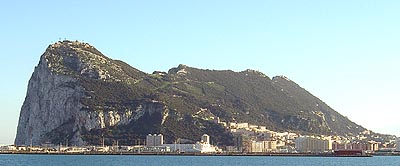
\includegraphics[width=\textwidth]{chapterthreename/figures/Rock_of_Gibraltar_northwest.jpg}
\tiny Source: Wikipedia
\end{figure}







% Chapter 4
%%
%% UW CBE Thesis: chapterfourname/chapterfourname.tex
%% Written by Ankur Gupta, Sep 1, 2013
%% Departament of Chemical and Biological Engineering
%% University of Wisconsin-Madison
%% Copyright (c) Ankur Gupta, 2014
%%
%% License: GPL v3. See LICENSE.
%%

% This is Chapter 4. Are you more than half way there?
% Keep going.
\chapter{Chapter Four Title}
\label{chap:chapterfourname}
\doublespacing

\section{Citations}
\label{sec:chapterfourname:citations}

Let's talk about citations. Ideally, you want to create a \texttt{.bib} file 
for your thesis. Avoid naming this bib file \texttt{thesis.bib} because it might 
get deleted\footnote{Murphy's Law\index{Murphy's Law} is especially powerful while writing 
a thesis. That's a fact. Always keep a current backup.}.
This thesis template comes with a file named \texttt{citations.bib}. 
Alternatively, you can store all your citations for all your latex projects 
in a common location. In Unix systems, this location is usually at 
\begin{code}
~/texmf/bibtex/bib/
\end{code}


\section{History of \LaTeX}
\label{sec:chapterfourname:history_of_latex}

\LaTeX~\cite{lamport:1986} is a document preparation system based on 
\TeX~\cite{knuth:1999}. \TeX was created by Donald Knuth, who is known 
for the multi-volume work such as~\citet{knuth:1997}.



\section{All about Radium}
\label{sec:chapterfourname:all_about_radium}
\index{radium}

As promised, we talk about ``radium'' again. We discussed ``radium'' 
in \chaptertwoname{} as well. And, as discussed, we need to index ``radium'' 
here again. 




% Chapter 5
%%
%% UW CBE Thesis: chapterfivename/chapterfivename.tex
%% Written by Ankur Gupta, Sep 1, 2013
%% Departament of Chemical and Biological Engineering
%% University of Wisconsin-Madison
%% Copyright (c) Ankur Gupta, 2014
%%
%% License: GPL v3. See LICENSE.
%%

% This is Chapter 5. You're now over the hump.
% Drive it home.
\chapter{Chapter Five Title}
\label{chap:chapterfivename}
\doublespacing

\section{Defining shortcuts}
\label{sec:chapterfivename:defining_shortcuts}

You will notice that I have a \texttt{shortcuts.tex} file in this thesis template folder. 
This file is then \texttt{input}ted in the file \texttt{uwcbethesis-config.tex}. 
The \texttt{shortcuts.tex} file contains many shortcuts that are going to be used 
repeatedly throughout in the thesis. For example, \verb+\chaptertwoname{}+ is a 
shortcut defined in \texttt{shortcuts.tex} file. \\

I have also defined many math symbols that I have to use repeatedly. The following 
equations use these commands. \\

The following equation describes a $n$-dimensional random vector, $\bfX$
\begin{align}
\bfX \sim \fN \left( \mu, \Sigma \right)
\end{align}
distributed normally with mean vector $\mu$ and covariance matrix $\Sigma$. The 
probability density of $\bfX$ is given by 
\begin{align}
f_{\bfX}(\bfx) = \frac{1}{(2\pi)^{\frac{n}{2}} \abs{\Sigma}^{\frac{1}{2}}}\text{ } e^{-\frac{1}{2} (\bfx-\mu)^{T} \Sigma^{-1} (\bfx-\mu)}
\end{align}



\section{Using \texttt{uwcbethesis-config.tex}}
\label{sec:chapterfivename:using_config_file}

Instead of typing out your name, department, title of your thesis, etc. 
this thesis template defines this data all at once in the file named
\texttt{uwcbethesis-config.tex}. Please make use of these commands instead 
of repeatedly typing out the data. Not only does this help reduce the number 
of typographical errors, it enforces homogeneity. This thesis template uses 
the commands defined in this config file. 




% Chapter 9
%%
%% UW CBE Thesis: conclusion/conclusion.tex
%% Written by Ankur Gupta, Sep 1, 2013
%% Departament of Chemical and Biological Engineering
%% University of Wisconsin-Madison
%% Copyright (c) Ankur Gupta, 2014
%%
%% License: GPL v3. See LICENSE.
%%

% And, you're done. It isn't that difficult once you start.
% Congratulations!
% You deserve it.
\chapter{Conclusions and future directions}
\label{chap:conclusions}
\doublespacing

\section{Contributions}
\label{sec:contributions}
% You don't need to list every chapter in this section. Instead, point 
% out the concepts, ideas, and everything new that you did. 
% You can refer to the chapters and remind the reader of your thesis 
% that these particular chapter contain your original contributions.

\noindent \textbf{Contribution One}. In \chaptertwoname{}, I present 
a new method to do somethimg great. This method has solved this problem 
which was not previously solved. \\


\noindent \textbf{Contribution Two}. In Chapters\ref{chap:chapterthreename} and 
\ref{chap:chapterfourname}, I present some more new stuff. The work done by 
others was great but more work was required, which I did in these chapters. \\

\noindent \textbf{Contribution Three}. In \chapterfivename{}, I present my 
final contribution. My masterpiece. \\

\section{Future research directions}
\label{sec:future_research_directions}

\noindent \textbf{Future research One.} More research is required in this area. 
In \chaptertwoname{} I solve some of these problems but there is more work to be 
done. \\

\noindent \textbf{Future research Two.} More research is required in this area. 
I recommend that this method be adopted. \\

\noindent \textbf{Future research Three.} More research is required in this area. 
I hope someone continues my work. \\

%---------------------------------------------

\appendix
%%
%% UW CBE Thesis: appendixA/appendixA.tex
%% Written by Ankur Gupta, Sep 1, 2013
%% Departament of Chemical and Biological Engineering
%% University of Wisconsin-Madison
%% Copyright (c) Ankur Gupta, 2014
%%
%% License: GPL v3. See LICENSE.
%%

% Appendices are easy.
\chapter{Appendix A Title}
\label{app:A}

This is an appendix. You should use an appendix for material which is important to 
present to the audience but which would distract the audience from the message 
if it were included in the main text. \\

An example is a long proof which is not central to the discussion in your main text. 
Another example is some software code that you think illustrates an idea. 
I would advise you not put large amounts of software code in the appendix because 
it is rather useless for the audience. People would use your code if it's available 
in digital form. Nobody wants to digitize your code. You can put a link to your 
code in your thesis. 


\section{Section One}
\label{sec:appA:section_one}

Appendices can contain sections. Appendices are like chapters as you can see. 


\section{Section Two}
\label{sec:appA:section_two}

Another section in the appendix.





%---------------------------------------------
%% Bibliography
%%
%% UW CBE Thesis: frontmatter/BibliographyPage.tex
%% Written by Ankur Gupta, Sep 1, 2013
%% Departament of Chemical and Biological Engineering
%% University of Wisconsin-Madison
%% Copyright (c) Ankur Gupta, 2014
%%
%% License: GPL v3. See LICENSE.
%%

% Add Bibliography to TOC
\phantomsection
% \refstepcounter{dummy}
\addtocontents{toc}{\protect\vspace{\beforebibskip}} % Set Bibliography a little apart
\addcontentsline{toc}{chapter}{\tocEntry{\bibname}}

\bibliographystyle{plainnat}
\bibliography{citations}


% This page should end now
\cleardoublepage
%---------------------------------------------



%---------------------------------------------
%% Index
%%
%% UW CBE Thesis: frontmatter/IndexPage.tex
%% Written by Ankur Gupta, Sep 1, 2013
%% Departament of Chemical and Biological Engineering
%% University of Wisconsin-Madison
%% Copyright (c) Ankur Gupta, 2014
%%
%% License: GPL v3. See LICENSE.
%%


% Add Index to TOC
\phantomsection
% \refstepcounter{dummy}
\addcontentsline{toc}{chapter}{\tocEntry{Index}}


\printindex


% This page should end now
\cleardoublepage
%---------------------------------------------


%---------------------------------------------
%% Vita
\singlespacing
%%
%% UW CBE Thesis: frontmatter/VitaPage.tex
%% Written by Ankur Gupta, Sep 1, 2013
%% Departament of Chemical and Biological Engineering
%% University of Wisconsin-Madison
%% Copyright (c) Ankur Gupta, 2014
%%
%% License: GPL v3. See LICENSE.
%%


% UW requirement: No Vita requirement but it's usual in my research group.
% Add a PDF bookmark. Need to do this because this page is not in TOC
% \pdfbookmark[0]{Vita}{vita}


% Add Vita to TOC
\phantomsection
% \refstepcounter{dummy}
\addcontentsline{toc}{chapter}{\tocEntry{Vita}}

% This is required to keep the quote above and the text below on the same page
\begingroup
\let\clearpage\relax
\let\cleardoublepage\relax
\let\cleardoublepage\relax



\chapter*{Vita}

\myName{} was born in the city of Kingsport, King's Landing. 
He then went to college to study. Then he did internships. 
Then he decided to come to this university to do his PhD. 
He won these awards. \\

After graduation, he is going to join the Night's Watch at 
The Wall as the Lord Commander. \\

\vspace{1ex}
\noindent Permanent Address: Kingsport, King's Landing\\

\vspace{1ex}
\noindent This dissertation was prepared by the author with \LaTeXe\xspace using his \texttt{uwcbethesis} template~\footnote{Feel free to remove this line.}



\endgroup 

% This page should end now
\cleardoublepage
%---------------------------------------------

\end{document}

